By offering a generic way to represent the knowledge in a domain,
Ontology simplifies the accumulation and share of various kinds of
knowledge among people or software agents. At the same time, it allows
automatic analysis and utilization of knowledge through high-level
declarative logic programming, thanks to its description logic
foundation.  These properties make it potentially valuable for
facilitating program analysis which is essentially about reasoning
about the knowledge related to a program. 

%% This section first gives an overview of the idea of using
%% ontology for program analysis. It then lists the critical challenges
%% for materializing the idea into a practical framework.

%\subsection{Overview}

\begin{figure}[t]
\centering
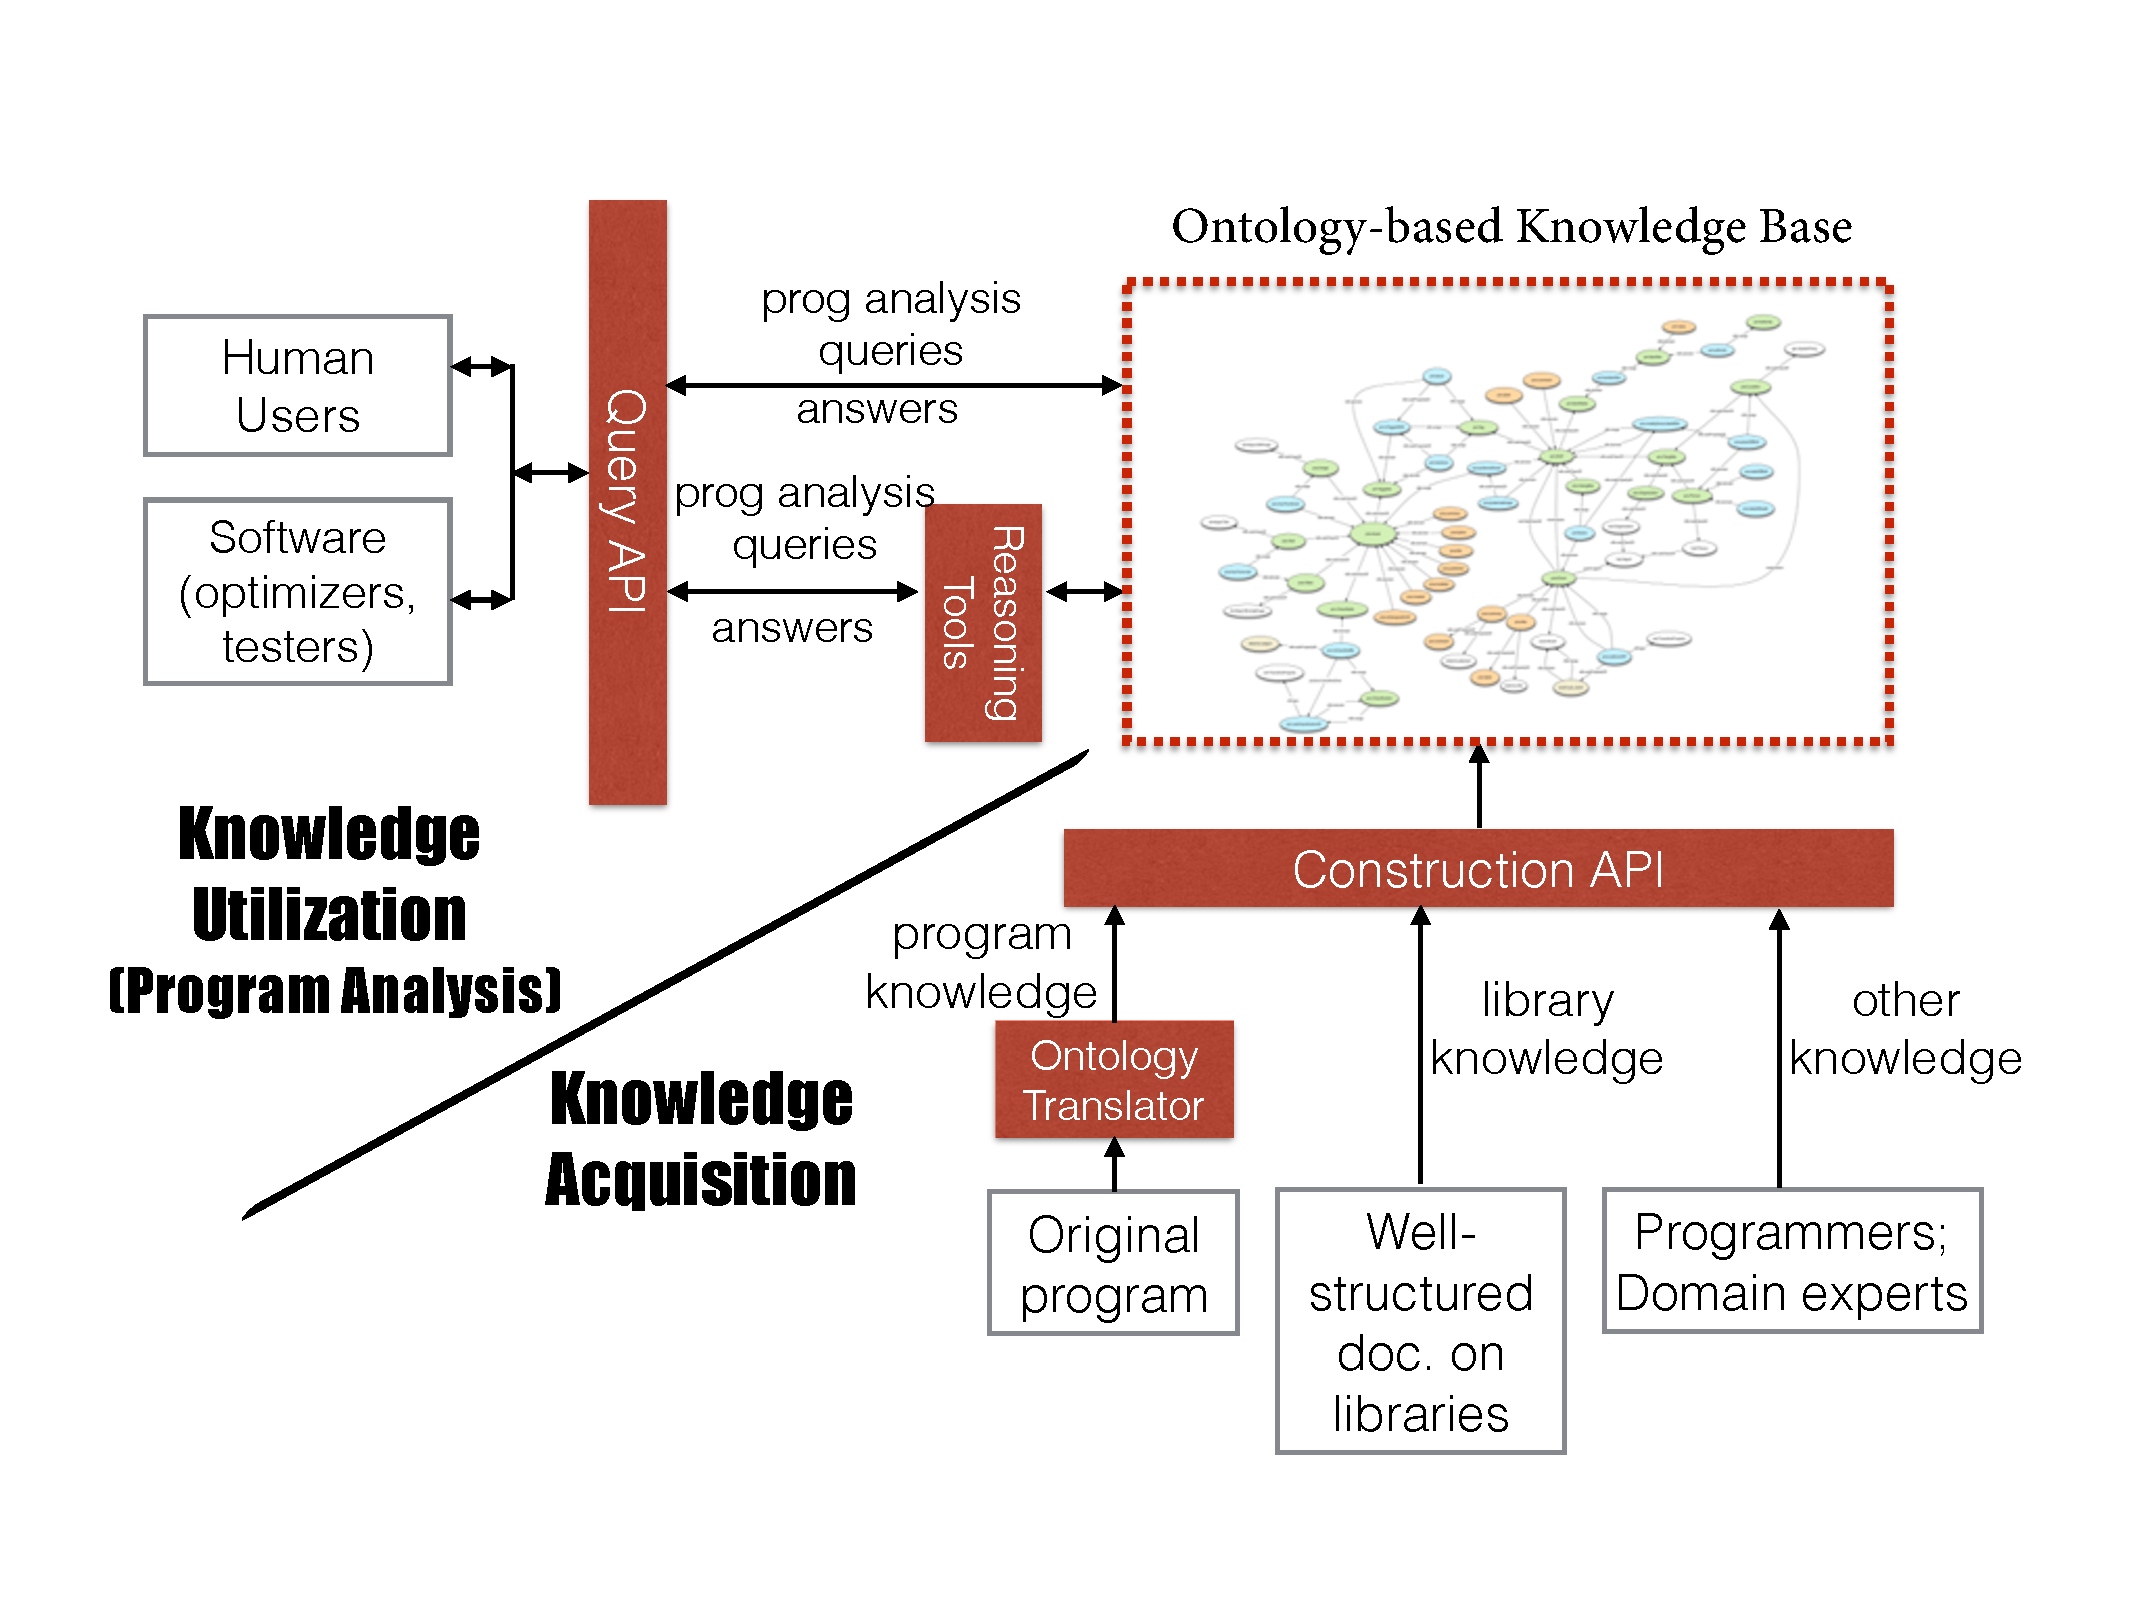
\includegraphics[width=.9\textwidth]{graph/overview.pdf}
\caption{Overview of using ontology for program
  analysis.}\label{fig:overview}
\end{figure}

Figure~\ref{fig:overview} illustrates the basic idea of ontology-based
program analysis. It centers around a knowledge base built upon
ontology.  The knowledge base may consist of the basic knowledge about
the code of the target program, as well as other knowledge (e.g.,
architecture attributes) relevant to the program analysis. An {\em
  ontology converter}, equipped with a parser, derives the basic
program knowledge from the code of the program, expresses the
knowledge in a standard format, and puts it into the knowledge
base. This basic knowledge may include the structures and components
(control blocks, data structures, etc.) of the program. In addition,
the knowledge base may include some knowledge that could be imported
about some libraries, or directly inputted by a domain expert on some
properties they know about the program or the architecture the program
is to run on (for the purpose of optimizations).

Built on top of description logic, ontology-based program analysis
keeps the conveniences of declarative program analysis. Rather than
writing thousands of lines of code inside a complex compiler, users
can simply write some logic queries about the kind of properties
(e.g., which loops are canonical loops) of the program that they want
to know. These queries should follow some ontology query APIs. The
APIs will then return the answers that are automatically obtained from
the ontology-based knowledge base. Processing of complex queries can
leverage many existing ontology reasoning
tools~\cite{wielemaker2011,tsarkov2006fact++}.  Users
of the ontology-based knowledge base can be humans as well as software
agents (e.g., tools for program optimizations or testing.)

\vspace*{.1in}
\noindent{\bf Example} We use canonical loop analysis to illustrate
how the idea of ontology-based program analysis works. A canonical
loop is a type of well-structured loop conforming to specifications as
shown in Figure~\ref{fig:canonical}.  Because of its regular
structure, it has been the focus of many studies on parallelization
and loop
optimizations~\cite{kandemir1999improving,LiaoSemantic-aware2010,DaMata2013}.

\begin{figure}[h]
\centering
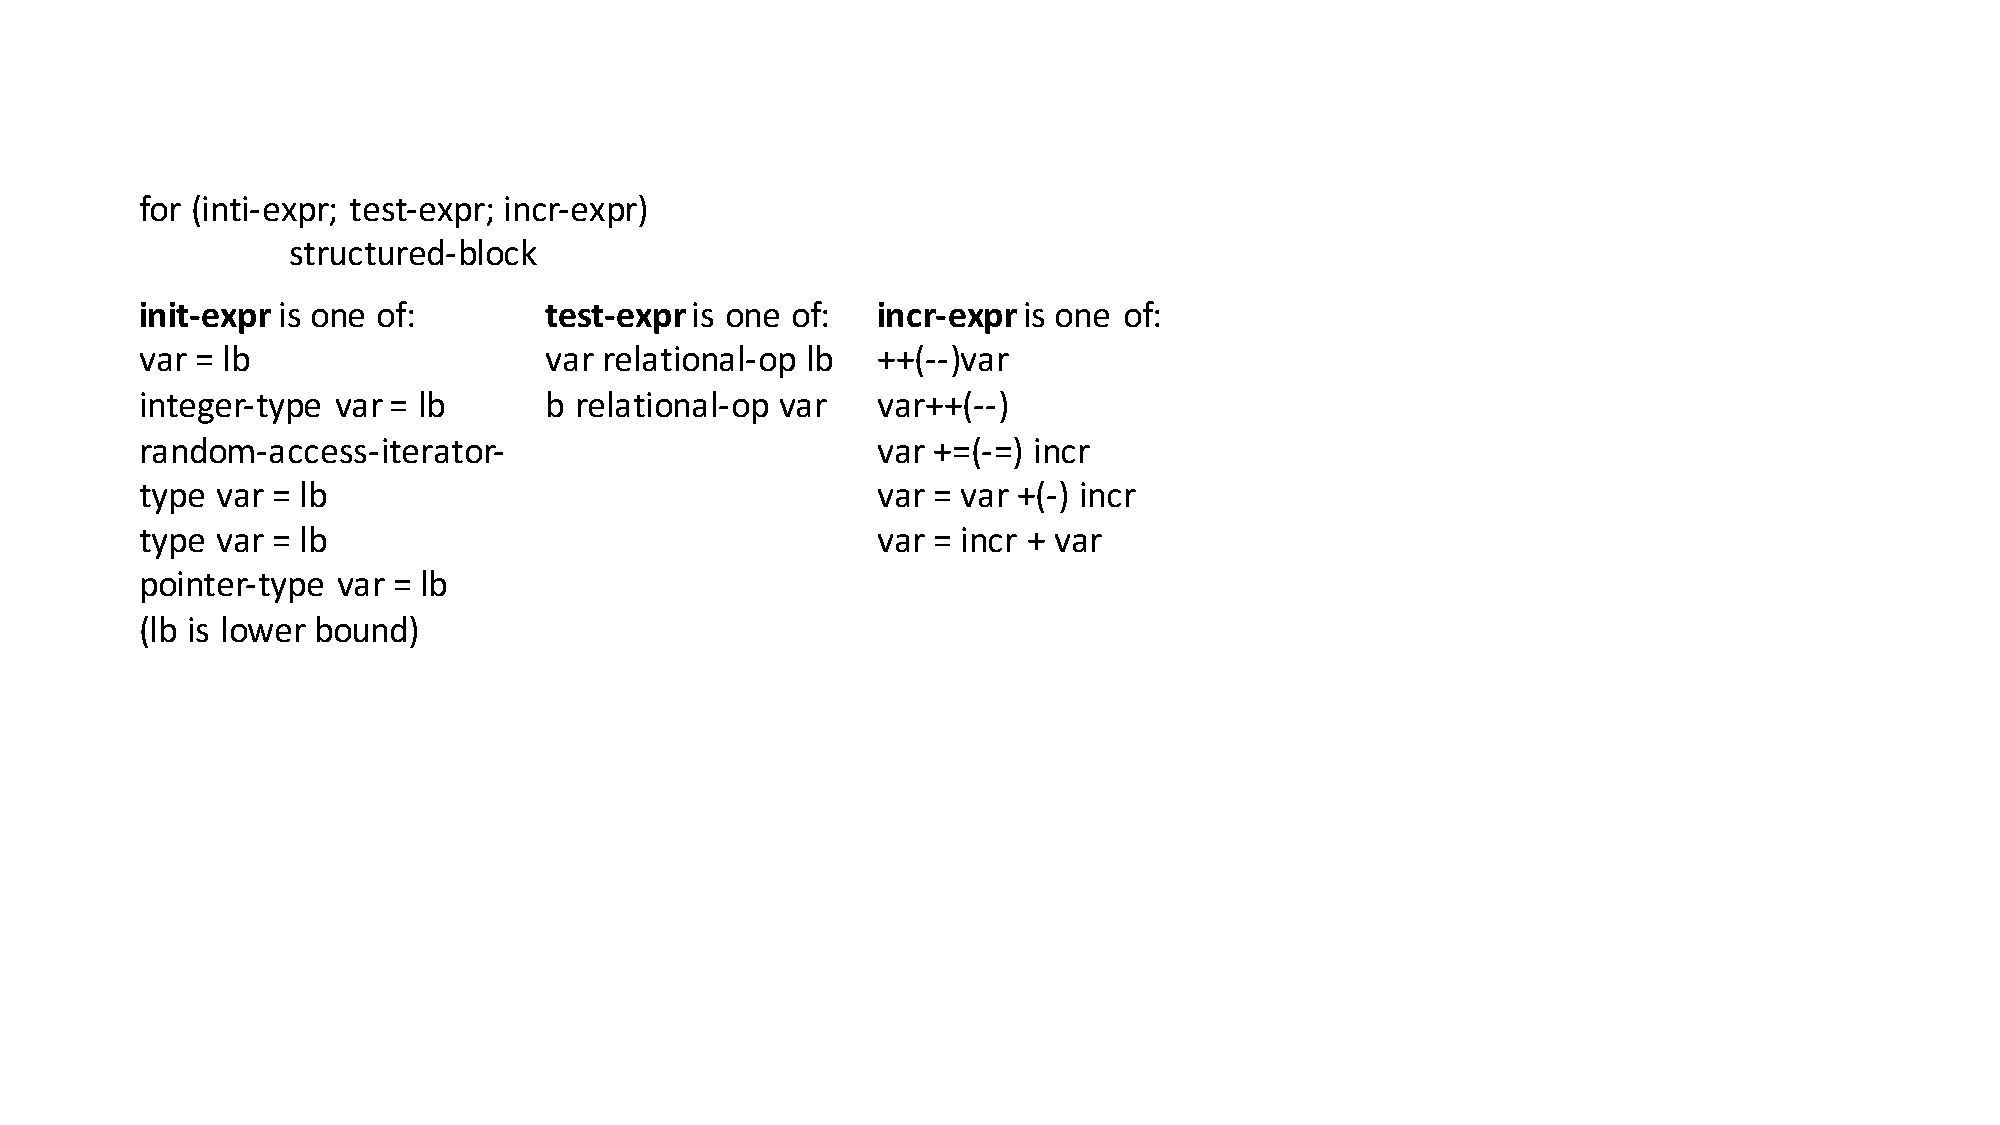
\includegraphics[width=.7\columnwidth]{graph/cl-def.pdf}
\caption{Specification of a canonical loop (derived from OpenMP
  manual~\cite{openmp13}.)
  %\TODO{remove boxes, put the three kinds of expr definitions into one single row below the ``for'' loop code.}
}
\label{fig:canonical}
\end{figure}

%An important program analysis (e.g., in ROSE~\cite{ROSE} and ??
%compilers)
The goal of {\em canonical loop analysis} is to recognize whether a
loop is in a canonical form.  Traditional implementations of the
analysis (e.g., the implementation in the ROSE compiler~\cite{ROSE})
contains hundreds of lines of code for examining the IR of a loop. The
code is tied to a particular internal data structure of the chosen
compiler, hard to port to another compiler or maintain.

In a
traditional program analysis development, the task requires an
insertion of a separate pass over some intermediate representation of
the whole program, which may need the development of thousands of
lines of code. For example, in the ROSE compiler~\cite{ROSE} (a
source-to-source compiler broadly used in High Performance Computing),
the pass works on an Abstract Syntax Tree (AST). To analyze the code
at that level, a programmer needs to implement many lines of code
written in procedural languages (C/C++).  The canonical loop analysis
in the ROSE compiler consists of 380 lines of source code for examining
the representations of the structure of each loop and check them
against the conditions in Figure~\ref{fig:canonical}.
%\TODO{add back the canonical figure using imperative codes}

In ontology-based program analysis, the process is simpler. The
programmer needs to invoke some provided ontology converter on the
code of the target program. An ontology-based knowledge base is then
produced to capture the program constructs, components, and their
relations.  The programmer then just needs to use a declarative logic
programming language to describe rules governing the forms that a
canonical loop should conform. Treating those rules as queries on the
ontology of the program, existing logic reasoners can then
automatically find all the canonical loops in the target program.
%\TODO{We should give sample ontology triplets and a few declarative analysis rules here. Otherwise readers cannot understand this.}
For example, a fragment of C code is shown in Listing~\ref{code:id}.
\begin{lstlisting}[numbersep=-8pt,firstnumber=0,
xleftmargin=.1\columnwidth,
xrightmargin=.1\columnwidth, float,
caption=Example C code fragment, label=code:id]
  // s.c
  int a = 0;
  int foo() {
   for (int i = 0; i < 10; i++) {
    a = a + i;
   }
  }
\end{lstlisting} 
The code's corresponding ontology representation is shown in Listing~\ref{code:onto_repr}.
Each line is a triple of a subject, a predicate and an object.
The numbers in the subjects are the line and column numbers for the begining and ending positions of a language construct in the source code. 
\begin{lstlisting}[xleftmargin=.1\columnwidth,
xrightmargin=.1\columnwidth, float,
caption=Sample ontology for C snippet, label=code:onto_repr]
('3:1,5:1', rdf:type, 'ForStatement')
('3:6,3:14', rdf:type, 'VariableDecl')
('3:6,3:10', rdf:type, Variable')
('3:1,5:1', 'hasForInit', '3:6,3:14')
('3:1,5:1', 'hasForTest', '3:17,3:22')
('3:1,5:1', hasForIncr', '3:25,3:27')
('3:1,5:1', hasBody', '3:30,5:1')
\end{lstlisting}
%\begin{lstlisting}[xleftmargin=.05\columnwidth, 
%xrightmargin=.05\columnwidth, float=h,
%caption=Sample ontology triples, label=ont:c_frag]
%...
%:334_3_342_3 rdf:type c:ForStatement .
%:334_3_342_3 c:hasParent :333_1_348_1 .
%:334_3_342_3 c:hasForInit :334_8_334_16 .
%:334_3_342_3 c:hasForTest :334_18_334_30 .
%:334_3_342_3 c:hasForIncr :334_33_334_38 .
%:334_3_342_3 c:hasBody :334_41_342_3 .
%... % omitted
%\end{lstlisting}
The different program constructs can be easily extracted by Prolog queries like those in Listing~\ref{code:sample_rule}.
\begin{lstlisting}[xleftmargin=.1\columnwidth,
xrightmargin=.1\columnwidth, float,
caption= Sample analysis rules, label=code:sample_rule]
isForStatement(Loop) :-
 rdf(Loop, rdf:type, c:ForStatement).
hasForInit(Loop, InitExpr) :-
 rdf(Loop, c:hasForInit, InitExpr).
\end{lstlisting}


Allowing the use of logic programming, ontology-based program analysis
inherits the productivity benefits of declarative program
analysis. More importantly, it overcomes the three aforementioned
shortcomings of existing declarative program analysis by leveraging
Ontology for standardizing the concept definitions in a domain and the
flexible representation of various sources of knowledge. 

%As
%shown in Figure~\ref{fig:loopProlog} (which will be further explained
%in Section~\ref{sec:exp}), the description can be nearly as simple as the
%English description in Figure~\ref{fig:canonical}. After that, the
%programmer just needs to put in a simple query in the Ontology Query
%API, asking the ontology reasoner to find all loops meeting the
%canonical loop conditions. The reasoner can soon return all the
%answers with the options of various visualizations of the results.

%% Writing declarative program analyses over an ontology is more
%% productive than writing imperative program analyses over a compiler
%% IR.  The main reason is that declarative programming interface works
%% on high level concepts.  It is quicker to develop and easier to make
%% it right. In addition, it is easy to modify and extend; some updates
%% to the high-level descriptions would be mostly sufficient.  It is also
%% portable since the concepts and relations being operated upon are
%% generic terms in the domain, totally independent from any particular
%% compiler's internal data structures.

%% Although the idea of the new paradigm is relatively straightforward,
%% materializing it is much beyond a simple application of the Ontology
%% techniques. There are some open questions special to program analysis that
%% must be answered. We present them and our next section.

